\hypertarget{sagittarius}{%
\chapter{Sagittarius}\label{sagittarius}}

\hypertarget{overview}{%
\section{Overview}\label{overview}}

Sagittarius (Sgr) is a dwarf spheroidal (dSph) galaxy in the Milky Way. It was
the ninth dwarf satellite discovered in the Milky Way, and the last to be
discovered before the advent of digital surveys~\cite{simon_faintest_2019}. It
was identified in 1994 by Ibata et al.~\cite{ibata_dwarf_1994} as a dwarf
satellite in the constellation of Sagittarius (hence its name). The authors
then noted that it was the closest galaxy to the Milky Way of any known at the
time, and this has largely remained true to the present.  One quirk about Sgr
that was noted at the time was that it ``is elongated towards the plane of the
Milky Way, suggesting that it is undergoing some tidal disruption before being
absorbed by the Milky Way.'' This would turn out to be a very important
feature of Sgr to explain.

In the years since, many studies have been performed to try to understand and
quantify various properties of Sgr, like its mass, orbital time, and the
reason for its elongated shape. By 2000, it was believed that the elongation
was the result of tidal shearing~\cite{jiang_orbit_2000}, meaning that
accurately describing the orbital history of Sgr is essential. Further, this
means we can expect that the stripping of stars by tidal forces may play a
significant role in its evolution. Jiang and Binney~\cite{jiang_orbit_2000}
thus explored the parameter space for the initial mass and radius of Sgr,
finding that a wide range of parameters are possible, from an initial mass of
\(\sim 10^{11}\) M\(_\odot\) and Galactocentric distance of \(\gtrsim 200\)
kpc to mass \(\sim 10^9\) M\(_\odot\) and distance \(\sim 60\) kpc.

Shortly thereafter, Majewski et al.~used the Two Micron All Sky Survey (2MASS)
to map Sgr, forming the first canonical model of Sgr~\cite{majewski_two_2003}.
Their characterization of Sgr included a description of a \emph{stream} of
stars that had been tidally stripped from the progenitor, forming leading and
trailing ``tidal tails''.  These tails, they note, ``lie along a well-defined
orbital plane about the Galactic center.'' Moreover, they state that the lack
of precession in the tidal debris is indicative of a nearly spherical
gravitational potential for the Milky Way, recognizing the usefulness of the
Sagittarius stream as a potential measure of the gravitational potential.

We have included a reproduction of Figure 11 from~\cite{majewski_two_2003}, a
plot of a sample of Sgr debris stars in equatorial coordinates and in the
orbital plane. It can be seen in Figure~\ref{fig:majewski}. The core of Sgr
lies at approximately $(+20, -10)$ kpc in the orbital coordinates, with the
northern arm leading above it and the southern arc leading to the left.

\begin{figure}
    \centering 
    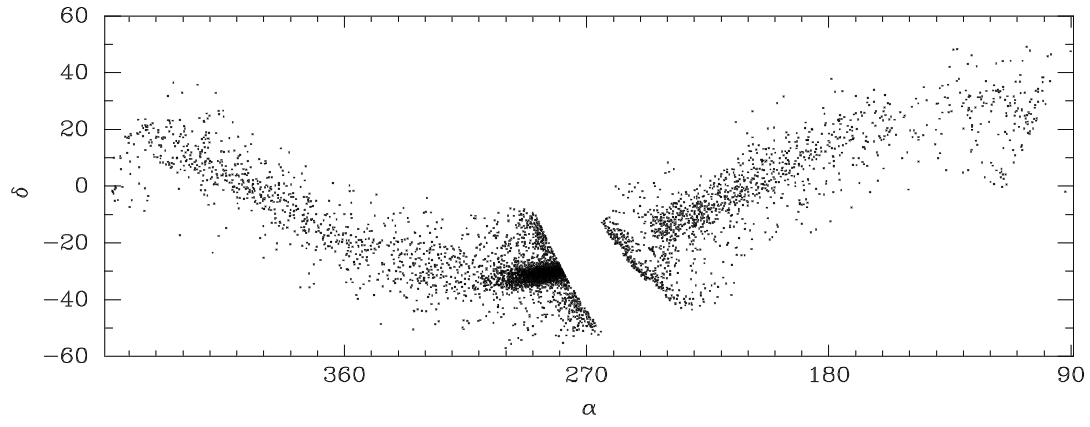
\includegraphics[width=0.7\linewidth]{figs/majewski2003-12.png}
    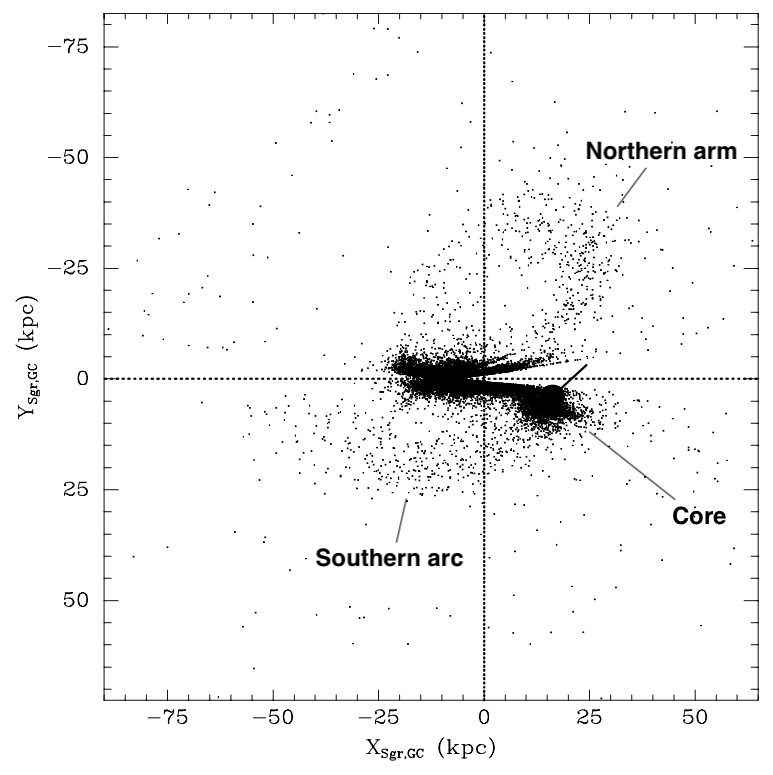
\includegraphics[width=0.45\linewidth]{figs/majewski2003-11.png}
    \caption{%
        Sgr debris in (top) equatorial coordinates and (bottom) in the orbital
        plane with the Galactic center at the origin. Reproduced from Figures
        11 and 12 of~\cite{majewski_two_2003}; labels added to bottom figure to
        match their Figure 9.
    }
    \label{fig:majewski}
\end{figure}

A similar work was performed by Belokurov et al.~in 2006, using the Sloan
Digital Sky Survey (SDSS)~\cite{belokurov_field_2006}. They found the tidal
stream of Sgr to be ``clearly visible'', and found the leading tidal arm to be
especially clear. We include their Figure 2, which shows a panoramic view of
the stream cutting together the 2MASS stars of Majewski et al.~with the SDSS
stars of Belokurov et al. This can be found in our
Figure~\ref{fig:belokurov2006}.

\begin{figure}
    \centering 
    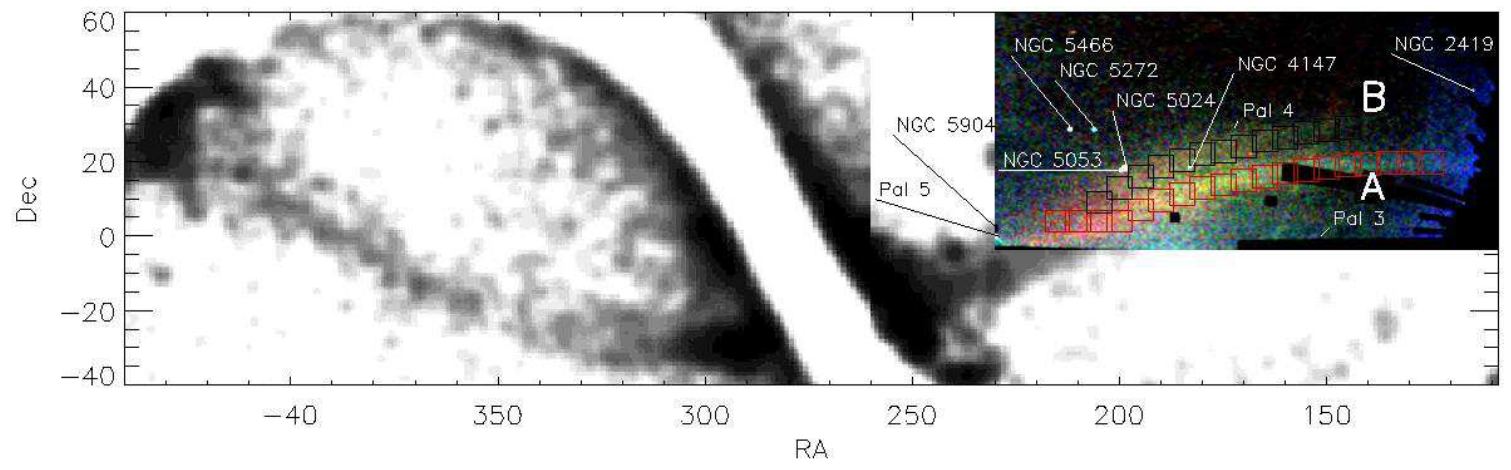
\includegraphics[width=0.95\linewidth]{figs/belokurov2006-2.png}
    \caption{%
        Sgr debris in equatorial coordinates, including both the 2MASS data
        from~\cite{majewski_two_2003} (in grayscale) as well as SDSS data
        from~\cite{belokurov_field_2006} (in color). Reproduced from Figure 2
        of~\cite{belokurov_field_2006}.
    }
    \label{fig:belokurov2006}
\end{figure}

The picture of Sagittarius as tidally disrupted with debris forming a long
streaming arc about the Milky Way would turn out to be well-supported by
further observations and studies. In the ensuing years, more studies were
performed to improve the model and more accurately quantify the properties of
the galaxy. We note in particular the work of Kunder and
Chaboyer~\cite{kunder_distance_2009} who estimated the distance to Sgr to be
approximately 24.8 kpc.

% todo add a discussion of stream coordinates?

\hypertarget{modern-models}{%
\section{Modern models}\label{modern-models}}

The next major discovery in the history of Sagittarius was the 2010 Law and
Majewski model~\cite{law_sagittarius_2010}. This model became the first to
successfully satisfy the majority of existing constraints on the angular
position, distance, and radial velocity of the tidal debris streams. It did so
using a triaxial Milky Way halo; in other words, it dropped the typical
assumption that the Milky Way halo is axisymmetric in the Galactic plane. One
prediction of note from this model is that the current bound mass of Sgr is
approximately \(2.5 \times 10^8\) M\(_\odot\). To obtain this, they use an
initial mass of \(6.4 \times 10^8\) M\(_\odot\) with an infall orbit for
around 8 Gyr in a fixed Galactic gravitational potential. It is worth noting
that this initial mass lies in the régime where dynamical friction is small
and the effects of tidal stripping on the Sgr progenitor are relatively
small~\cite{dierickx_predicted_2017}.

The resulting distribution of stars is shown in Figure~\ref{fig:law}. We
reproduce their plots of the debris stream in terms of heliocentric
coordinates and Galactocentric distances in the orbital plane. The coloring
corresponds to the time at which the debris was stripped from Sgr. (Green is
between the first and third apocenters, cyan between the third and fifth,
magenta between the fifth and seventh, and orange later than the seventh.)
Notice as well that they predict \textit{two} wraps for both the leading
(``L'') and trailing (``T'') stream arms.

\begin{figure}
    \centering 
    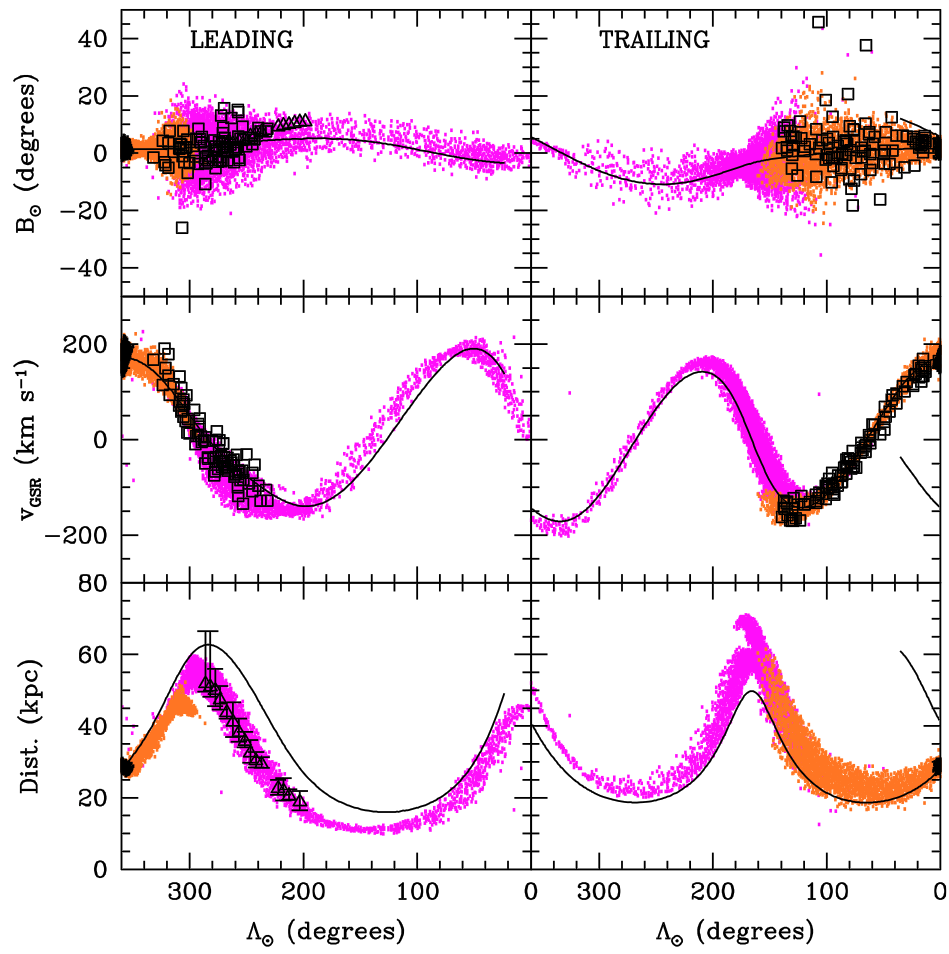
\includegraphics[width=0.45\linewidth]{figs/law2010-6.png}
    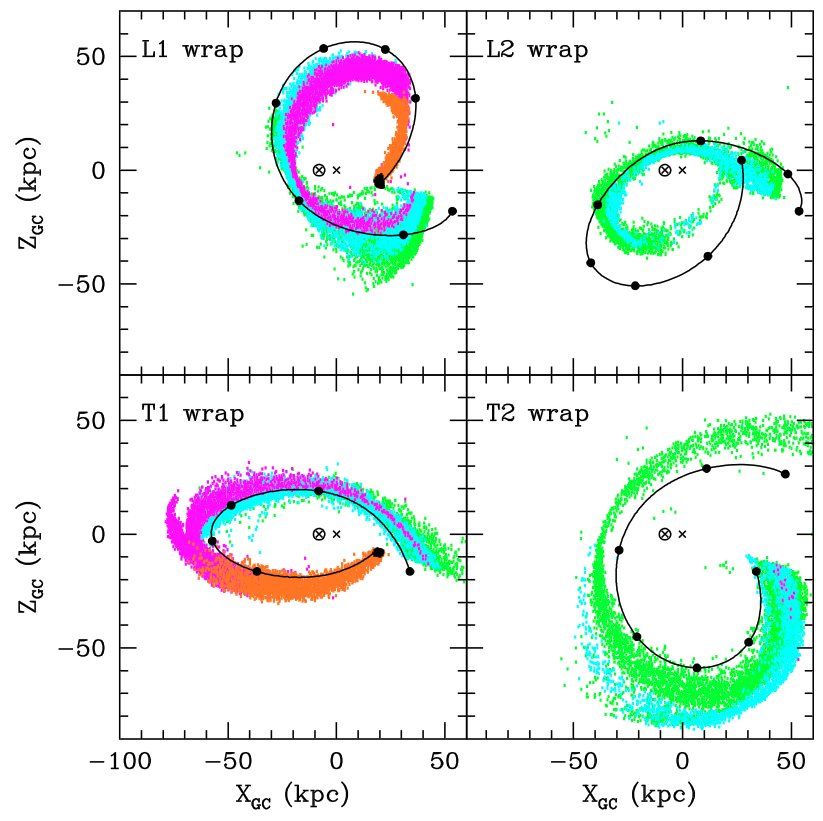
\includegraphics[width=0.45\linewidth]{figs/law2010-8.png}
    \caption{%
        Sgr stellar debris streams according to the Law and Majewski 2010
        model. On the left, debris stripped in the last $\sim 3$ Gyr is shown
        in terms of stream and heliocentric coordinates. On the right, the
        first two wraps of the leading (``L'') and trailing (``T'') stream
        arms are shown in the orbital plane. These plots are reproduced from
        Figures 6 and 8 of~\cite{law_sagittarius_2010}.
    }
    \label{fig:law}
\end{figure}

Shortly thereafter came the model of Purcell et
al.~\cite{purcell_sagittarius_2011}. In their model, they explicitly account
for the impact of the infall of Sagittarius on the evolution of the Milky Way
disk, pointing out that all then-existing models of Sgr assume that its
effects on the Galactic disk morphology are negligible. They found that Sgr
created ``significant perturbations to the outer disk'' with noticeable
effects on the evolution of the inner spirality. In their model, Sgr is
represented as beginning with halo mass \(10^{10.5}\) M\(_\odot\) at a
Galactocentric radius of 80 kpc in the Galactic plane. In order to account for
tidal stripping that would have occurred between the infall of Sgr past the MW
virial radius and the starting position they choose, they truncate the initial
halo at the instantaneous Jacobi radius, \(r_t = 23.2\) kpc. We note that such
methods may produce qualitatively accurate representations of Sgr but are
unlikely to accurately reflect the true orbital history of Sgr.

The resulting stream debris is shown in Figure~\ref{fig:purcell}. We show again
both the stream in terms of heliocentric coordinates and in the orbital plane in
terms of Galactocentric distances. We focus in particular on the ``light Sgr''
subplot of the Galactocentric figure. The figures show qualitatively similar
patterns to the model of Law and Majewski~\cite{law_sagittarius_2010}, including
the ``L1'' and ``T1'' wraps.

\begin{figure}
    \centering 
    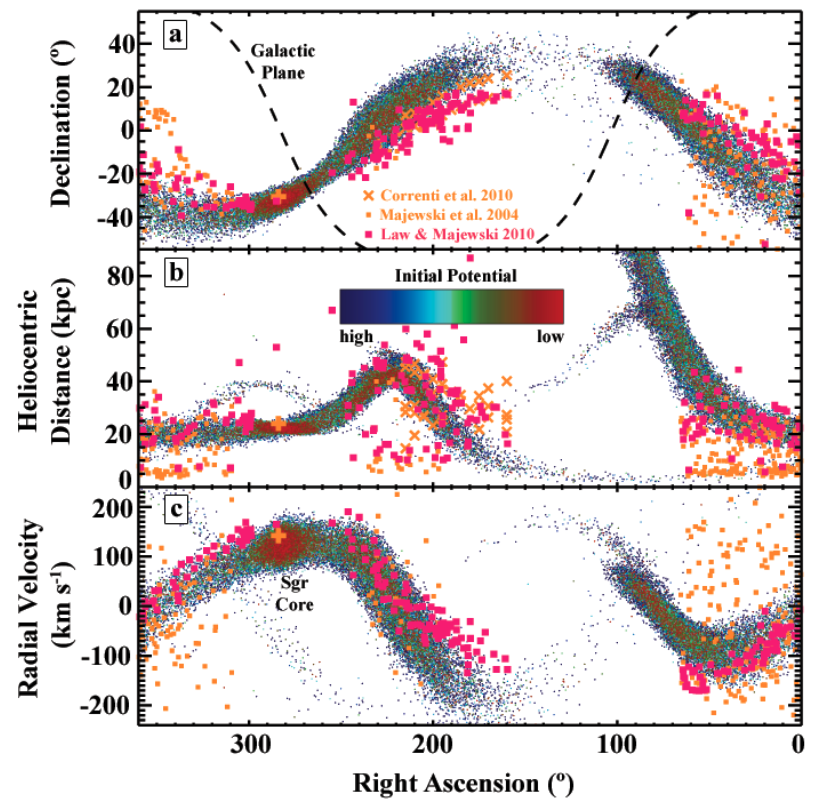
\includegraphics[width=0.41\linewidth]{figs/purcell2011-3.png}
    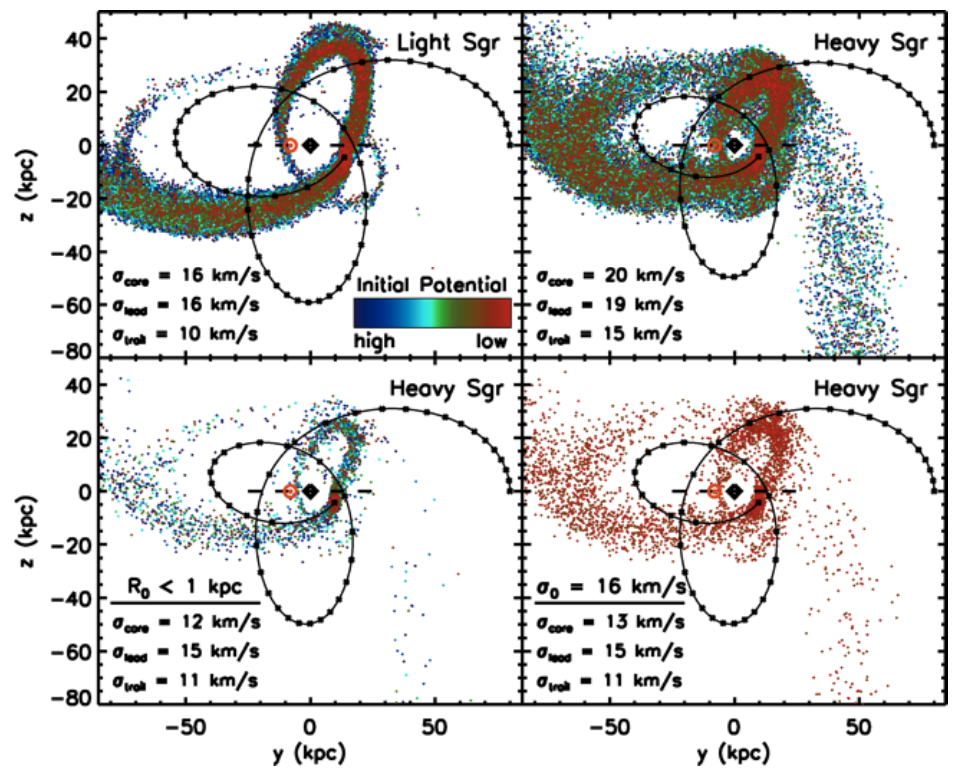
\includegraphics[width=0.5\linewidth]{figs/purcell2011-s4.png}
    \caption{%
        Sgr stellar debris streams according to the Purcell et al.~2011 model.
        On the left, debris is shown in terms of equatorial and heliocentric
        coordinates. On the right, the debris is shown in terms of
        Galactocentric distances in the orbital plane. We pay particular
        attention to the ``light Sgr'' subplot and note that the debris
        appears to contain approximately the same shape as the ``L1'' and
        ``T1'' wraps of the Law model. Figures reproduced from Figures 3 and
        S4 of~\cite{purcell_sagittarius_2011}.
    }
    \label{fig:purcell}
\end{figure}

As such, the status until quite recently was that no existing Sagittarius
model could accurately account for a live Milky Way potential, the effects of
dynamical friction, and the early infall of Sgr at Galactocentric radii of
more than 60-80 kpc.  In 2017, however, a new model which sought to solve all
these problems was introduced by Dierickx and
Loeb~\cite{dierickx_predicted_2017}.  They simulated the infall of Sagittarius
starting from its first crossing of the Milky Way virial radius approximately
8 Gyr ago using a live Milky Way gravitational potential and accounting for
the full effects of dynamical friction.  To find the best-fit model, they
began by performing a parameter search with a fast and simple semi-analytic
model.  They then used these best-fit parameters in a full, high-resolution
N-body simulation.

The resulting simulation is able to reproduce both the leading and trailing
stream arms to good agreement with both observed data and past models.
Moreover, they note that the resulting model is the first to accurately
reproduce existing data for debris observed 100 kpc away. The model also
predicts the existence of an extension to the stream, including ``the
existence of several arms of the Sgr stream extending to hundreds of
kiloparsecs.'' They note that this predicted structure matches the positions
of the two most distant stars known in the Milky Way halo and serves as a
testable prediction for data from future sky surveys.

This model is the one that we have (approximately) chosen to adopt for our
simulations. The specific differences between our model and theirs will be
elucidated in Section~\ref{pipeline-and-parameters}.  Dierickx and Loeb
represent the Milky Way halo using a Hernquist distribution with total mass
\(1.25 \times 10^{12}\) M\(_\odot\) and scale radius 38.35 kpc.  The Milky Way
disk follows an exponential profile with mass \(8.125 \times 10^{10}\)
M\(_\odot\), scale length 3.5 kpc, and scale height 0.525 kpc.  They also use
a Hernquist bulge with mass \(1.25 \times 10^{10}\) M\(_\odot\) and scale
length 0.7 kpc.  In their model, Sagittarius has a Hernquist halo with total
mass \(1.3 \times 10^{10}\) M\(_\odot\) and scale radius 9.81 kpc.  It has an
exponential disk with mass \(6 \times 10^{8}\) M\(_\odot\), scale length 0.85
kpc, and scale height 0.1275 kpc, and a Hernquist bulge with mass \(5.2 \times
10^{8}\) M\(_\odot\) and scale length 0.17 kpc.

As before, we include plots of the resulting stellar debris, both in terms of
heliocentric coordinates and Galactocentric distances in the orbital plane.
These plots are given in Figure~\ref{fig:dierickx}. In this case, the familiar
stream structure is once again reproduced, but with the inclusion of a
significant extension to the stream arms far beyond the two wraps considered
by Law and Majewski. The resulting distribution also appears to approximately
reproduce the distributions of observed stars (observational data shown in
black).

\begin{figure}
    \centering 

    \begin{subfigure}{0.43\textwidth}
        \centering
        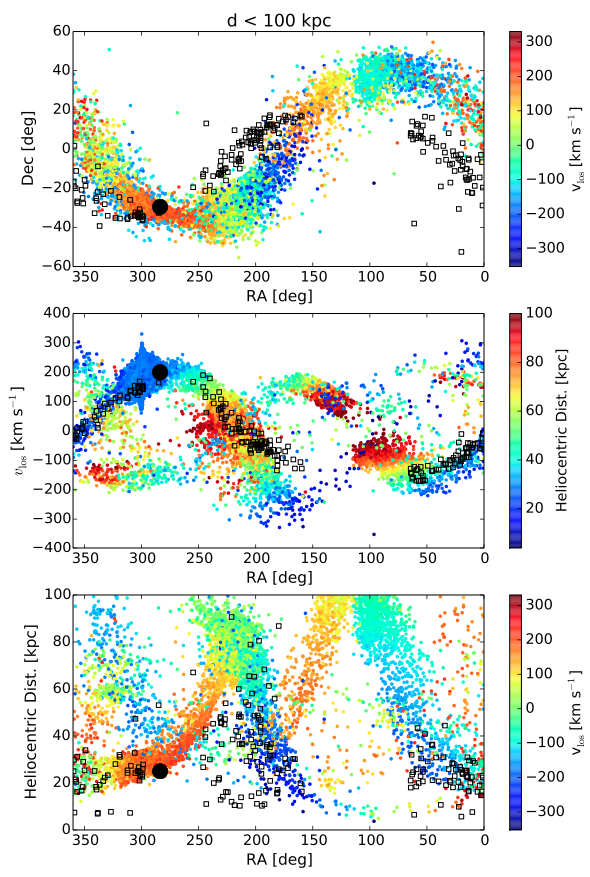
\includegraphics[width=\textwidth]{figs/dierickx2017-10.png}
    \end{subfigure}
    \begin{subfigure}{0.52\textwidth}
        \centering
        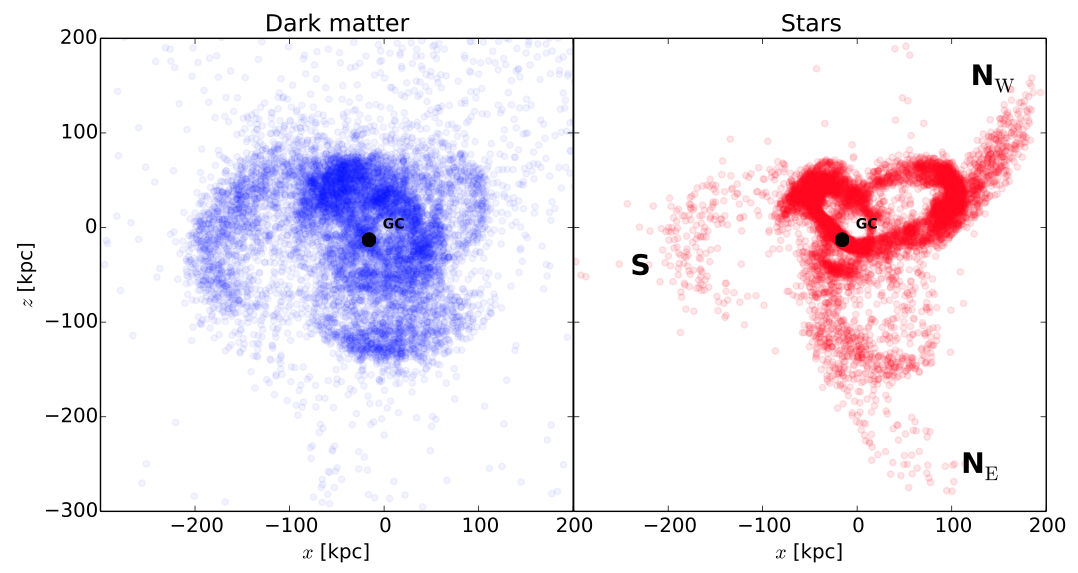
\includegraphics[width=\textwidth]{figs/dierickx2017-8.png}
        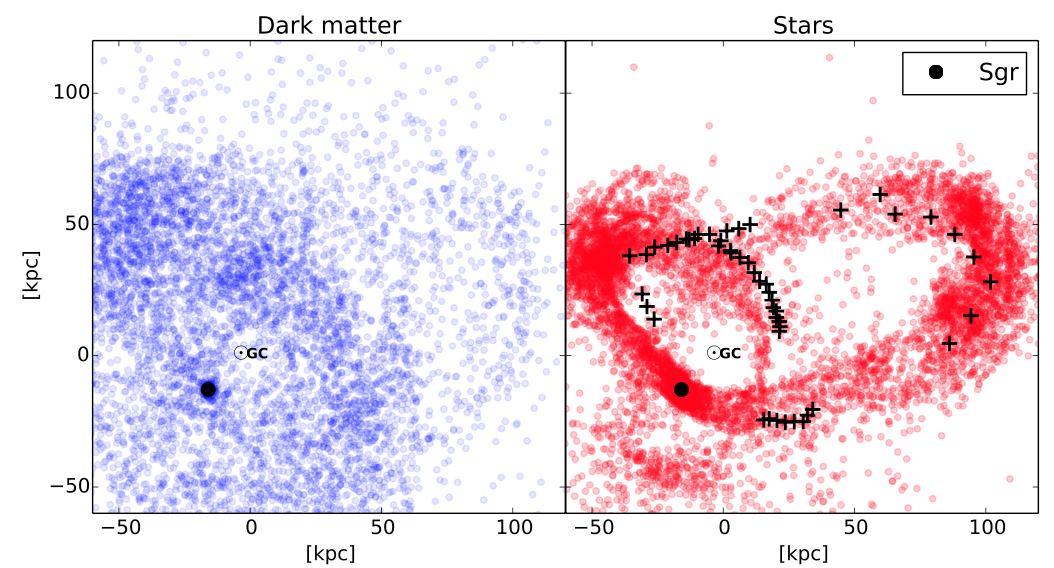
\includegraphics[width=\textwidth]{figs/dierickx2017-9.png}
    \end{subfigure}

    \caption{%
        Sgr stellar debris according to the Dierickx and Loeb 2017 model. As
        before, we show the stream in equatorial and heliocentric coordinates
        on the left. On the right is the stream (and associated dark matter
        particles) in terms of Galactocentric distances in the orbital plane.
        The right top subfigure shows the full distributions, while the right
        bottom subfigure zooms into the more observationally relevant region.
        Comparisons to observed Sgr stars are also shown in black. Plots
        reproduced from Figures 8, 9, and 10
        of~\cite{dierickx_predicted_2017}.
    }
    \label{fig:dierickx}
\end{figure}
